\section{MGnify amplicon pipeline}\label{sec:MGnify}
Version 5.0 of the amplicon pipeline was enhanced by incorporating classification of fungi based on the internal transcribed spacer (ITS) regions, in addition to the small subunits (SSU) and large subunits (LSU) based classifications that were already present in the previous version~\cite{mitchell_mgnify_2020}. If the data consists of paired-end reads, the amplicon pipeline initiates by merging the reads using SeqPrep v1.2, as shown in the complete amplicon flowchart in \Cref{fig:amplicon-pipline}. Subsequently, the merged reads undergo quality control, using Trimmomatic v0.36 to trim low-quality sequencing regions. Following quality control, the rRNA-prediction subworkflow is executed. The subworkflow comprises a search against Rfam v13.0 SSU and LSU models utilizing cmsearch v1.1.2. Furthermore, MAPseq v1.2.3, in conjunction with the SILVA v132 database, conducts taxonomic classification. The outputs consist of abundance tables visualized using Krona v2.7.1 as pie charts. The charts and outputs of the pipeline are accessible via the MGnify website~\cite{noauthor_mgnify_nodate-23} or through the API~\cite{mitchell_mgnify_2020}.

\begin{figure}[H]
  \centering
  \subfloat{{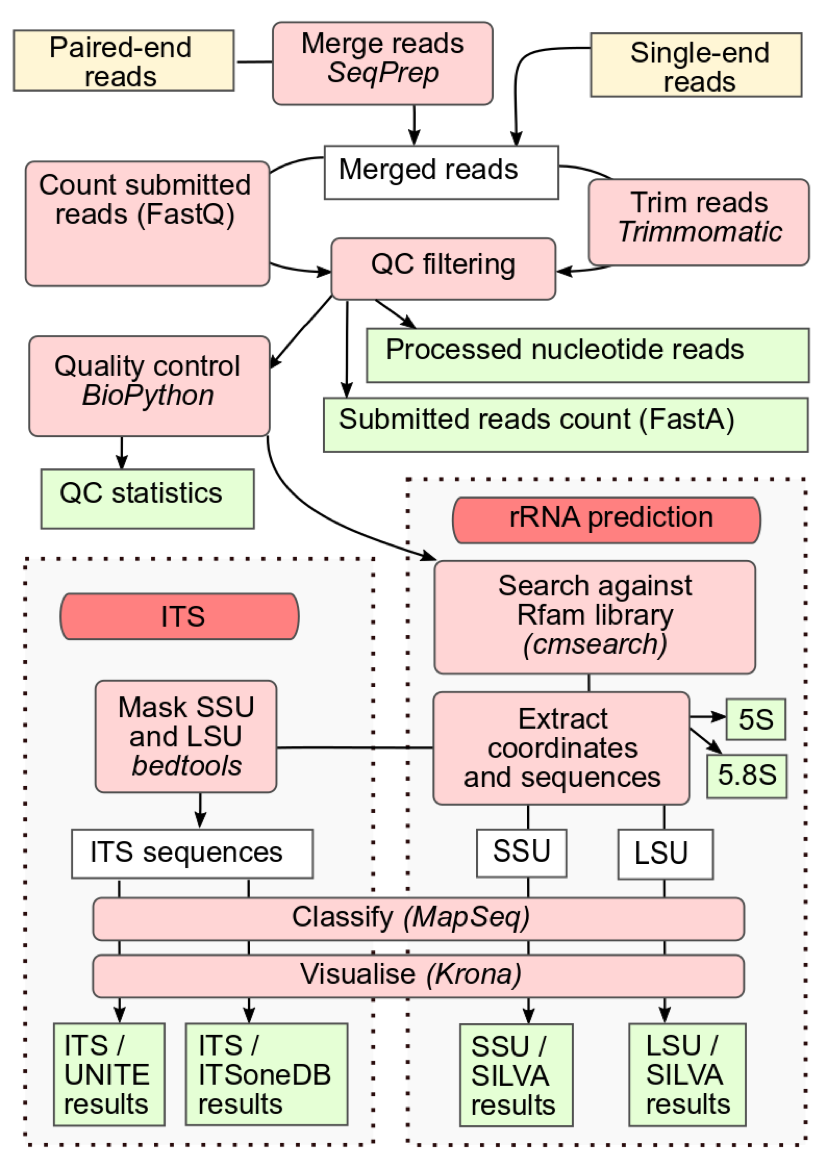
\includegraphics[scale=0.7]{figures/mgnify-workflow-wb.png} }}%
  \captionof{figure}[MGnify's amplicon pipeline]{\textbf{MGnify's amplicon pipeline v5.0}. The flowchart illustrates the workflow of MGnify's amplicon pipeline, with the rRNA-prediction subworkflow enclosed within a dotted box on the right~\cite{noauthor_mgnify_nodate-25}.} \label{fig:amplicon-pipline}%
\end{figure}